\chapter{Is light a particle or a wave?}

You may have heard that light is both a particle and a wave, and that this is paradoxical. We want you to get a clear sense of why physicists have come to this wild conclusion, and continue to practice working with the scientific cycle that we have presented.

\section{Learning goals}

\begin{itemize}
	\item Make careful predictions based on hypotheses and a given experimental setup.
	
	\item Gain a clear sense of how light behaves like a particle, and how it behaves like a wave.
\end{itemize}

\section{Lab Team Roles}

Decide which team members will hold each role this week: facilitator, scribe, technician, skeptic. If there are three members, consider having the skeptic double with another role. Consider taking on a role you are less comfortable with, to gain experience and more comfort in that role.

Additionally, if you are finding the lab roles more restrictive than helpful, you can decide to co-hold some or all roles, or thinking of them more like functions that every team needs to carry out, and then reflecting on how the team executed each function.

\section{Observation experiment: describing waves and particles}

In order to make predictions in the testing experiments with light, it will be helpful to determine what properties waves and particles have in more obvious situations, so that these properties can be applied to less obvious situations with light.

\subsection{Goal}

Describe patterns of behavior of waves and particles that can be used to differentiate between them.

% target observations for particles:
% - when two of them travel to intersect, they collide and change direction
% - can only be emitted or absorbed as discrete units

% target observations for waves:
% - when two of them travel to intersect, they overlap and continue undisturbed
% - continuous transmission of energy


\subsection{Available equipment (simulated)}

\begin{itemize}
	\item Particle box: box where particles move towards each other and interact (Simulation:  \url{https://phet.colorado.edu/sims/html/collision-lab/latest/collision-lab_all.html} (Select ``Explore 2D''))

	\item Ripple tank: tank of shallow water with set of plungers (to create waves) and walls that obstruct the path of waves (Simulation: \url{http://www.falstad.com/ripple/})
	
	\item String attached to an oscillator (Simulation: \url{https://phet.colorado.edu/sims/html/wave-on-a-string/latest/wave-on-a-string_en.html})
\end{itemize}

\subsubsection{What happens when their paths intersect?}

{\color{red} This might not have enough discovery about interference leading to dark fringes. This also might not have enough discovery that particles travel in straight lines while waves spread out like wavelets.}

\begin{steps}
	\item In the particle box, \textbf{observe and record} what happens when the two particles approach each other and interact. How are their motions different after the interaction?
	
	\item In the ripple tank, watch the wave crests (light color) expand away from the source, a plunger pushing down and up in the water.
	
	\item Click anywhere in the tank to touch your finger into the water momentarily and create a ripple (a single wave crest). \textbf{Observe and record} what happens when the ripple approaches each wave crest and interacts. How are the ripple and wave motions different after the interaction?

	\item Summarize the difference between particles and waves in this case.

\end{steps}

\subsubsection{How do they deliver energy?}

\begin{steps}
	\item With the wave on a string simulation, click ``loose end'' on the right side, then click and drag the wrench to see how it moves the string.
	
	\item Select ``Oscillate'' on the left side of the screen. Reduce the amplitude to about 0.2 cm. Reduce the frequency to exactly 1.47 Hz. Reduce the damping to ``None''.
	
	\item Press ``Restart'' to reset the string to neutral.
	
	\item Watch what happens as the wave delivers energy to the ring at the right. Does the wave deliver energy continuously or in short bursts? Is there a minimum amplitude needed to start the ring in motion?
	
	\item In contrast to this, consider the following example of particles: imagine that you have a bag of basketballs and a friend is sitting on a chair on wheels, which is resting on a carpet. If you toss the ball gently to them, they don't budge at all. But if you toss a ball fast enough, it pushes them back. Does this deliver energy continuously or in short bursts? And if you keep tossing balls gently to them, will that ever get them moving?

	\item Summarize the difference between particles and waves in this case.

\end{steps}

\section{Testing experiment: is light a particle or wave?}

\subsection{Goal}

For the two situations below (light incident on metal and light incident on slits), test the following hypotheses:
\begin{enumerate}[label=(\Alph*)]
	\item\label{lpw:hyp:part} Light is made of particles.
	\item\label{lpw:hyp:wave} Light is made of waves.
\end{enumerate}

\subsection{Situation 1: light shining on metal}

\subsubsection{Assumptions}

\begin{itemize}
	\item Light travels with different wavelengths.
	
	\item Light with a shorter wavelength (higher frequency) carries more energy.
	
	\item Metals have particles called ``electrons'' in them that can absorb energy from light. Once an electron absorbs a certain amount of energy, it is emitted from the metal and gains kinetic energy.
\end{itemize}

\subsubsection{Available equipment (simulated)}

The following equipment is available as a simulation here: \url{https://phet.colorado.edu/en/simulation/legacy/photoelectric}

\begin{itemize}
	\item An evacuated glass tube, inside of which are two metal plates connected by a conducting wire.
	
	\item A lamp that can emit light at different, controllable wavelengths and at different, controllable intensities, aimed at only the left plate
	
	\item A method of seeing electrons that are floating inside the tube (in real life these are not directly visible)
	
	\item A method of measuring the electric current produced in the wire (electric current is proportional to the number of electrons arriving at the right plate per second)
\end{itemize}

\subsubsection{Steps}

\begin{steps}
	
	\item Before turning on the lamp, determine what each hypothesis \ref{lpw:hyp:part} and \ref{lpw:hyp:wave} predicts will happen when the wavelength and intensity are varied. \textbf{Record the two predictions.}
	
	\item Develop an experimental procedure that will allow you to collect the data you need to compare to the predictions. \textbf{Record this procedure.}
	
	\item Collect and record your relevant data.
	
	\item Compare the experimental outcome to the predictions and determine which, if any, of the predictions agree with the outcome, and to what degree.
\end{steps}


\subsection{Situation 2: light shining on two small slits}

%{\color{red} Should this be two small light bulbs instead, so it's more similar to the previous observation?}

Consider the situation in Figure~\ref{lpw:fig:2slit-setup}.

\begin{figure}
	\centering
	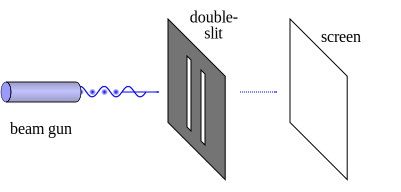
\includegraphics[width=0.6\textwidth]{light-particle-wave/Double-slit-setup.pdf}
	\caption{Experimental setup. Note that the light emitted from the beam gun (or laser) is broad enough to go through both slits.}\label{lpw:fig:2slit-setup}
\end{figure}

\begin{steps}
	\item Determine what each hypothesis \ref{lpw:hyp:part} and \ref{lpw:hyp:wave} predicts the screen will look like. Where are the dark and bright regions?
	
	\item Ask your TA for the experimental result that was done using a red laser.
	
	\item Compare the experimental outcome to the predictions and determine which, if any, of the predictions agree with the outcome, and to what degree.
\end{steps}



%Consider two lamps that are close to each other, of a single 

\subsection{Conclusion}

\begin{steps}
	\item Given the results from Situations 1 and 2 above, what judgment can you make about the hypotheses?
\end{steps}

\section{Group dynamics}

\begin{steps}
	\item Write a 100--200 word reflection on group dynamics and feedback on the lab manual. Address the following topics: who did what in the lab, how did you work together, what successes and challenges in group functioning did you have, and what would you keep and change about the lab write-up?
	
	\item Write a paragraph reporting back from each of the four roles: facilitator, scribe, technician, skeptic. Where did you see each function happening during this lab, and where did you see gaps?
\end{steps}

\section{Report checklist and grading}

The lab grade consists of 3 points for each of seven scientific ability rubric rows (the 5 listed above, which apply just to that section, as well as F1 and F2, applied to the entire report), and 9 points for providing evidence in the lab report of completing all steps of the lab, including answering every question, for a total of 30 points.